\section{Preliminary}	%\section{Overview of algorithms}
\label{sec-problem}


In this section, we introduce some basic concepts for trajectory simplification.
For convenience, notations used are summarized in \mytable{tab:notations}.

%\stitle{Points}. A data point is defined as a triple $P(x, y, t)$, which represents that a moving object is located at {\em longitude} $x$ and {\em latitude} $y$ at {\em time} $t$. Note that these data points can be viewed as points in the x-y-t 3D Euclidean space.

\stitle{Point}. A data point is defined as a triple $P(x, y, t)$ \myblue{in a suitable coordinate system, representing that a moving object is located at {$(x, y)$} at time $t$. 
In practice, a raw data point collected from an end device of some Global Navigation Satellite System is usually defined by geo-spatial data standards (e.g., World Geodetic System 84 coordinates) with a format of ({\em longitude, latitude, altitude, time}). In this article, these raw data points are projected to a x-y-t 3D Euclidean space (called map projection \cite{Hargitai:Projection}) during trajectory simplification.}

%in  Euclidean space

%like Global Positioning System (GPS), BeiDou Navigation Satellite System (BDS), GLObal NAvigation Satellite System (GLONAS) and Galileo

%{A data point could also be defined as a quadruple $P(x, y, z, t)$, where $z$ is {\em altitude}. However, to our knowledge, the current trajectory simplification algorithms all consider the x-y spatial information only, and the height information, if concerning, is treated as an independent dimension that could be simplified by piece-wise linear approximation methods \cite{Agarwal:Metric, ORourke:Fitting, Keogh:online, Luo:Streaming, Xie:Stream,Elmeleegy:Stream}.}


%We first introduce basic notations.
\stitle{Trajectory}. A \textit{trajectory} $\dddot{\mathcal{T}}\left[P_0, \ldots, P_n\right]$ is a sequence of points in a monotonically increasing order of their associated time values (\ie $P_i.t < P_j.t$ for any $0\le i<j\le n$). %Note that data points can be viewed as points in a three-dimension Euclidean space.
Intuitively, a trajectory is the path (or track) that a moving object follows through space as a function of time~\cite{physics-trajectory}.

\stitle{Directed line segment}. A directed line segment (or line segment for simplicity) $\mathcal{L}$ is defined as $\vv{P_{s}P_{e}}$, which represents the closed line segment that connects the start point $P_s$ and the end point $P_e$.
Note that here $P_s$ and $P_e$ are different points that may not in a trajectory $\dddot{\mathcal{T}}$.

%, and hence, we also use notation $\mathcal{R}$ instead of $\mathcal{L}$ when both $P_s$ and $P_e$ belong to $\dddot{\mathcal{T}}$.

For the projection of a directed line segment $\mathcal{L}$ on an \emph{x-y} 2D space, where $x$ and $y$ are the longitude and latitude, respectively, we also use $|\mathcal{L}|$ and $\mathcal{L}.\theta\in [0, 2\pi)$ to denote the length of $\mathcal{L}$ in the x-y 2D space, and its angle with the $x$-axis of the coordinate system $(x, y)$.  That is, the projection of a directed line segment $\mathcal{L}$ = $\vv{P_{s}P_{e}}$ on an \emph{x-y} 2D space is treated as a triple $(P_s, |\mathcal{L}|, \mathcal{L}.\theta)$.

%Intuitively, a trajectory can also be represented by a continuous $n$-pieces directed line segments (or line segment for simplicity) $\mathcal{L}_i$, $0\le i < n$, where  $\mathcal{L}_i = \vv{P_{i}P_{i+1}}$, represents the closed line segment that connects the start point $P_{i}$ and the end point $P_{i+1}$.

\stitle{Piece-wise line representation}. A \textit{piece-wise line representation} $\overline{\mathcal{T}}\left[\mathcal{L}_0, \ldots, \mathcal{L}_m\right]$ ($0< m \le n$) of a trajectory $\dddot{\mathcal{T}}\left[P_0, \ldots, P_n\right]$ is a sequence of continuous \textit{directed line segments} $\mathcal{L}_{i}$ = $\vv{P_{s_i}P_{e_i}}$ ($i\in\left[0,m\right]$) of $\dddot{\mathcal{T}}$ such that $\mathcal{L}_{0}.P_{s_0} = P_0$, $\mathcal{L}_{m}.P_{e_m} = P_n$ and  $\mathcal{L}_{i}.P_{e_i}$ = $\mathcal{L}_{i+1}.P_{s_{i+1}}$ for all $i\in\left[0, m-1\right]$.
Note that (1) each directed line segment in $\overline{\mathcal{T}}$ essentially represents a continuous sequence of data points in trajectory $\dddot{\mathcal{T}}$, (2) a piece-wise line representation is a simplified trajectory, {essentially the sequence of end points of all line segments}, {and (3) a point ($x$, $y$, $t$) on a spherical surface is  projected on a 2D flat plane in the piece-wise line representation.}


	\begin{table}
	\renewcommand{\arraystretch}{1.20}
	\vspace{-1ex}
	\caption{\small Summary of notations}
	\centering
	\footnotesize
	%\scriptsize
	\begin{tabular}{|c|l|}
		\hline
		{\bf Notations}& {\bf Semantics}   \\		\hline %\hline
		$P$ & a data point \\		\hline
		$\dddot{\mathcal{T}}$ & a trajectory $\dddot{\mathcal{T}}$ is a sequence of data points\\		\hline
		$\overline{\mathcal{T}}$&  {a piece-wise line representation of a trajectory $\dddot{\mathcal{T}}$}	\\		\hline
		$\mathcal{L}$ & a directed line segment  \\		\hline
		$\mathcal{M}$ & a distance metric of \ped, \sed or \dad \\		\hline
		$ped\left(P, \mathcal{L}\right)$ &  {the perpendicular Euclidean distance of point $P$ to line segment $\mathcal{L}$}	\\	\hline
		$sed\left(P, \mathcal{L}\right)$ & {the synchronous Euclidean distance of point $P$ to line segment $\mathcal{L}$} 	\\		\hline
		$dad\left(\mathcal{L}_1, \mathcal{L}_2\right)$ & {the direction-aware distance of line segment $\mathcal{L}_1$ to line segment $\mathcal{L}_2$} 	\\		\hline
		$\epsilon$ & an error bound \\		\hline
		$\mathcal{A}$ & a line simplification algorithm \\		\hline
		%\sector{} & a sector \\		\hline
		%		$\vv{A} \times \vv{B}$ & the cross product of (vectors) $\vv{A}$ and $\vv{B}$\\		\hline
		%		$\mathcal{H}(\mathcal{L})$ & The open half-plane to the left of $\mathcal{L}$ \\		\hline
		%		$\mathcal{R}$& a convex polygon \\		\hline
		%		$\mathcal{R}^*$ & the intersection of convex polygons \\		\hline
		%		$m$ & the maximum number of edges of a polygon\\		\hline
		%		$E^j$ & a group of edges labeled with $j$\\		\hline
		%		$g(e)$ & the label of an edge $e$ of polygons \\		\hline
		%		\circle{} & a synchronous circle\\		\hline
		%\cone{} & a spatio-temporal cone \\		\hline
		%		\pcircle{} & a cone projection circle \\		\hline
		%$\bigsqcap$ & intersection of geometries\\		\hline
		%$G$ &	the reachability graph of a trajectory\\		\hline
	\end{tabular}
	\label{tab:notations}
	\vspace{-1ex}
\end{table}


 For trajectory simplification, three distance metrics are commonly used, namely, the \emph{perpendicular Euclidean distance} (\ped), the \emph{synchronous Euclidean distance} \cite{Meratnia:Spatiotemporal} (\sed) and the \emph{direction-aware distance}\cite{Long:Direction, Zhang:Evaluation} (\dad).
%
Consider a data point $P$ and a directed line segment $\mathcal{L}$ = $\vv{P_{s}P_{e}}$.

\stitle{Perpendicular Euclidean distance}. The perpendicular Euclidean distance $ped\left(P, \mathcal{L}\right)$ of point $P$ to line segment $\mathcal{L}$ is $\min\{|PQ|\}$ for any point $Q$ on $\vv{P_{s}P_{e}}$.
%
{This definition is also called the \emph{tolerance-zone} error measure \cite{Daescu:metric,Barequet:3D,Chen:Space,Imai:Optimal,Melkman:Optimal}.}
{Note that in the field of computational geometry, (1) there is a slight variation of \emph{tolerance-zones}, called the \emph{infinite beam} or \emph{parallel-strip} criterion \cite{Daescu:metric,Chen:Space}, which is the perpendicular Euclidean distance of a point to a line, and (2) it is believed that tolerance-zones could produce a compressed version that better captures the features of the original path/curve \cite{Daescu:metric,Barequet:3D,Chen:Space}. If not otherwise specified, we use tolerance-zones to evaluate algorithms.}
%, the most natural definition of \ped~\cite{Barequet:3D}	
	
\stitle{Synchronous Euclidean distance}. The synchronous Euclidean distance $sed\left(P, \mathcal{L}\right)$ of point $P$ to line segment $\mathcal{L}$ is $|\vv{PP'}|$ that is the Euclidean distance from $P$ to its \textit{synchronized data point} $P'$ \wrt $\mathcal{L}$, where the synchronized data point $P'$ \wrt $\mathcal{L}$ is defined as follows:
(a) $P'.x$ = $P_s.x +  c\cdot\left(P_e.x - P_s.x\right)$,
(b) $P'.y$ = $P_s.y +  c\cdot\left(P_e.y - P_s.y\right)$ and
(c) $P'.t$ = $P.t$, where $c= \frac{P.t-P_s.t}{P_e.t-P_s.t}$.

{Synchronized points are essentially virtual points with the assumption that an object moves along a straight line segment from $P_s$ to $P_e$ with a uniform speed, \ie the average speed $\frac{|\vv{P_sP_e}|}{P_e.t-P_s.t}$ between points $P_s$ and $P_e$ \cite{Cao:Spatio,Lin:Cised}. Then the \emph{synchronized point} $P'$ of a point $P$ \wrt the line segment $\vv{P_sP_e}$ is the expected position of the moving object on $\vv{P_sP_e}$ at time $P.t$, obtained by a linear interpolation \cite{Cao:Spatio}. More specifically, a synchronized point $P'_i$ of $P_i$ ($s\le i < e$) \wrt the line segment $\vv{P_sP_e}$ is a point on $\vv{P_sP_{e}}$ satisfying ${|\vv{P_sP'_i}|} = \frac{P_i.t - P_s.t}{P_e.t - P_s.t}\cdot {|\vv{P_sP_e}|}$, which means that the object moves from $P_s$ to $P_e$ at an average speed $\frac{|\vv{P_sP_e}|}{P_e.t-P_s.t}$, and its position at time $P_i.t$ is the point $P'_i$ on $\overrightarrow{P_sP_{e}}$ having a distance of $\frac{P_i.t - P_s.t}{P_e.t - P_s.t}\cdot|\vv{P_sP_e}|$ to $P_s$~\cite{Cao:Spatio, Lin:Cised,Meratnia:Spatiotemporal, Chen:Fast, Zhang:Evaluation}.}

{Instead of directly using \sed,  \cite{Chen:Fast} introduces Local Integral Square \sed (\lissed, also called LSSD in \cite{Cao:Dots,Chen:Fast}) with $lissed(P_s,P_{s+k}) = \sum_{i=s}^{s+k-1} sed^2(P_i, \vv{P_sP_{s+k}})$. The most important feature of \lissed is that it can be computed in an incremental way, \ie given information about $lissed(P_s,P_{s+k})$, $lissed(P_s,P_{s+k+1})$ can be calculated in $O(1)$ time, such that algorithms using it (\eg~\bumr~\cite{Chen:Fast} and \dagots~\cite{Cao:Dots}) have lower time complexities compared with directly using \sed.
It is worth pointing out that (1) \lissed is  a special \sed-based \emph{error} measure rather than a new kind of \emph{distance} metric, (2) if the \lissed error bound of such an algorithm is set to $\epsilon^2$, then the maximal \sed error between the original and simplified trajectories is always not greater than $\epsilon$, and (3) the most recent algorithm directly using \sed, \ie~\cised, is very efficient, and has $O(n)$ time.}
%and (2) \lissed brings very different simplified trajectories compared with \sed
%{Besides, in order to speed up the simplification, a few algorithms \cite{Chen:Fast, Wu:Graph,Cao:Dots} alternatively use an accumulation of square \sed, named Local Integral Square Synchronous Euclidean Distance (\lissed) \cite{Chen:Fast}, as the error bound. \bumr~\cite{Chen:Fast} is such a batch algorithm, and \dagots~\cite{Cao:Dots} follows the ideas of \cite{Chen:Fast} and provides an online version. These \lissed-equipped algorithms ensure that any \lissed from data points to their representing line segment is limited by a preset \lissed error bound.}


\stitle{Direction-aware distance}. The direction-aware distance $dad\left(\mathcal{L}_1, \mathcal{L}_2\right)$ is the direction deviation from $\mathcal{L}_1$ to $\mathcal{L}_2$, \ie $\Delta\left(\mathcal{L}_1.\theta, \mathcal{L}_2.\theta\right) = \min\{|\mathcal{L}_1.\theta - \mathcal{L}_2.\theta|, 2\pi - |\mathcal{L}_1.\theta - \mathcal{L}_2.\theta|\}$.
{Note \dad differs from \ped and \sed in that it is a measure of angle differences, rather than Euclidean distances, and the temporal information is also lost when using \dad.}





We illustrate these notations with examples.

\begin{example}
	\label{exm-notations}
	Consider {Figure}~\ref{fig:dp}, in which
	%
	(1) $\dddot{\mathcal{T}}\left[P_0, \ldots, P_{10}\right]$ is a trajectory having 11 data points,
	%
    (2) the set of two continuous line segments $\{\vv{P_0P_4}$, $\vv{P_4P_{10}}$\}, the set of four continuous line segments $\{\vv{P_0P_2}$, $\vv{P_2P_4}$, $\vv{P_4P_7}$, $\vv{P_7P_{10}}$\} and the set of three continuous line segments $\{\vv{P_0P_4}$, $\vv{P_4P_5}$, $\vv{P_5P_{10}}$\} are three piece-wise line representations of trajectory $\dddot{\mathcal{T}}$,
	%
	(3) $ped\left(P_4, \vv{P_0P_{10}}\right)=|\vv{P_4P^*_4}|$, where $P^*_4$ is the perpendicular point of $P_4$ \wrt line segment $\vv{P_0P_{10}}$,
	%
	(4) For $P_4$, its synchronized point $P'_4$ \wrt $\vv{P_0P_{10}}$ satisfies $\frac{|\vv{P_0P'_4}|}{|\vv{P_0P_{10}}|} = \frac{P_4.t - P_0.t}{P_{10}.t-P_0.t} = \frac{4-0}{10-0}= \frac{2}{5}$,
	%
	(5) $sed\left(P_4, \vv{P_0P_{10}}\right)= |\vv{P_4P'_4}|$, $sed\left(P_2, \vv{P_0P_{4}}\right)= |\vv{P_2P'_2}|$ and $sed\left(P_7, \vv{P_4P_{10}}\right)$ $=$ $|\vv{P_7P'_7}|$,
	where points $P'_4$, $P'_2$ and $P'_7$ are the synchronized points of $P_4$, $P_2$ and $P_7$ \wrt line segments $\vv{P_0P_{10}}$, $\vv{P_0P_{4}}$ and $\vv{P_4P_{10}}$, respectively, and
    %
    (6) $dad\left(\vv{P_5P_6}, \vv{P_0P_{10}}\right)=\theta_{56}$ is the \dad of line segments $\vv{P_5P_6}$ to $\vv{P_0P_{10}}$.
\end{example}


\begin{figure}[tb!]
	\centering
	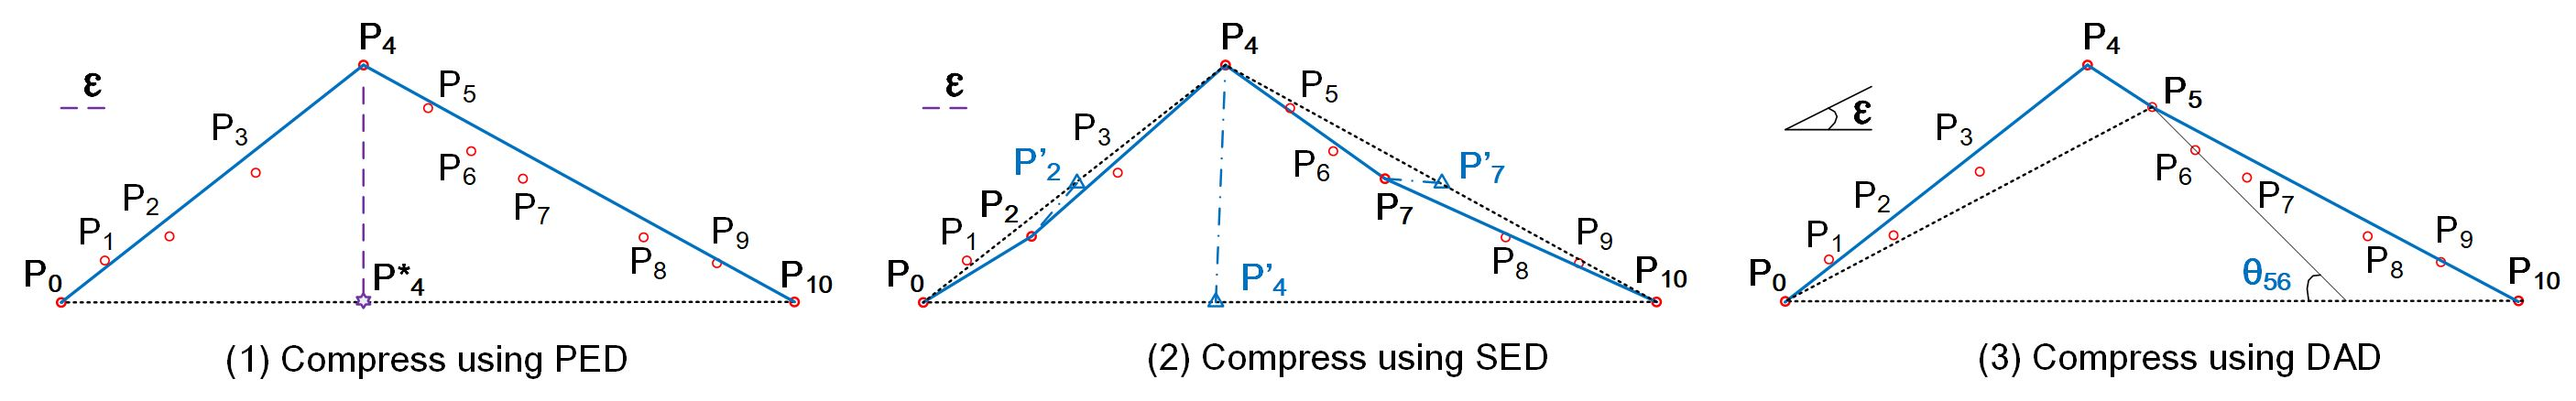
\includegraphics[scale=0.46]{Figures/Fig-DP.jpg}\vspace{-1ex}
	%\caption{\small A trajectory is simplified by algorithm \dpa using distance metrics \ped, \sed and \dad, respectively.}
	\caption{\small  A trajectory $\dddot{\mathcal{T}}[P_0, \ldots, P_{10}]$ with 11 points is compressed by the Douglas--Peucker algorithm \cite{Douglas:Peucker} using distance metrics \ped, \sed and \dad, respectively.}
		\vspace{-2ex}
	\label{fig:dp}
\end{figure}



%\stitle{Min-$\#$ problem}. Given a trajectory \trajec{T}$\left[P_0, \dots, P_n\right]$ and a pre-specified constant $\epsilon$, the \emph{min-$\#$} problem of trajectory simplification is to approximate the trajectory \trajec{T} with $\overline{\mathcal{T}}\left[\mathcal{L}_0, \ldots , \mathcal{L}_m\right]$ ($0< m \le n$), such that
%(1) on each of them the points $\left[P_{s_i}, \dots, P_{e_i}\right]$ are approximated by a line segment $\mathcal{L}_i = \vv{P_{s_i}P_{e_i}}$ with the maximum \ped or \sed \emph{error} of point $P_j$ (or \dad \emph{error} of line segment $|\vv{P_jP_{j+1}}|$) to line segment $\mathcal{L}_i$, $s_i \le j<e_i$,  less than $\epsilon$, and
%(2) $P_{s_i}$ and $P_{e_i} \in$ \trajec{T}.

%We finally introduce error bounded algorithms for trajectory simplification.

\stitle{{Trajectory simplification algorithms}}. {Given a trajectory \trajec{T}$\left[P_0, \dots, P_n\right]$ and a pre-specified bound $\epsilon$, a \emph{trajectory simplification algorithm} $\mathcal{A}$ using \ped (respectively, \sed and \dad) produces a piece-wise line representation $\overline{\mathcal{T}}\left[\mathcal{L}_0, \ldots, \mathcal{L}_m\right]$ ($0< m \le n$) by applying distance checking of \ped (respectively, \sed and \dad) with respect to $\epsilon$, such that for each $i\in[0, m]$, line segment $\mathcal{L}_i = \vv{P'_{s_i}P'_{e_i}}$ ($s_i < e_i$) approximately represents the sub-trajectory \trajec{T}$_i\left[P_{s_i}, \dots, P_{e_i}\right]$ of \trajec{T}.}

\stitle{{Error bounded algorithms}}. Given a trajectory \trajec{T}$\left[P_0, \dots, P_n\right]$ and a pre-specified bound $\epsilon$,
trajectory simplification algorithm $\mathcal{A}$ using \ped  (respectively, \sed and \dad) is \emph{error bounded} by $\epsilon$ if for each point $P_k$ ($k\in[0,n]$) in \trajec{T}, there exists a line segment $\mathcal{L}_i = \vv{P'_{s_i}P'_{e_i}}$ in $\overline{\mathcal{T}}$ with $s_i \le k \le e_i$ ($0\le i\le m$) such that the \ped distance $ped\left(P_k, \mathcal{L}_i\right)$  (respectively the \sed distance $sed\left(P_k, \mathcal{L}_i\right)$ and the \dad distance $dad\left(\vv{P_{k}P_{k+1}}, \mathcal{L}_i\right)$) is no more than  $\epsilon$.
%

Note that here {there is no need} to require that for all $i\in[0,m]$, points $P'_{s_i}$ and $P'_{e_i}$ of $\overline{\mathcal{T}}$ belong to the original trajectory \trajec{T}. That is to say, {data interpolations are allowed.}
